\section{Arquitectura de Comportamientos}

\subsection{Introducci\'on}
Como se dijo en las secciones anteriores, el objetivo de \'este trabajo
es desarrollar un robot aut\'onomo y reactivo que recolecte basura en un entorno
estructurado pero din\'amico, debido a que la arena ( lugar donde se mueve el robot )
es transitado por personas y es al aire libre.

En \'esta secci\'on de \emph{Arquitecturas de Comportamientos} se van
a detallar las acciones que deber\'a hacer el robot y c\'omo organizar las mismas
para cumplir la meta de recolectar basura y ser aut\'onomo, es decir, decidir por
s\'i mismo las acciones a realizar en cada momento y ser capaz de mantenerse cargado
para poder continuar recolectando.

En la secci\'on \ref{inv_prev} se analizar\'an
papers relacionados con este desarrollo, desde la forma de organizar los comportamientos,
la definici\'on y composici\'on de los mismos, hasta su implementaci\'on. En la secci\'on
\ref{arq_prop} se detallar\'a la arquitectura elegida para llevar a cabo y organizar los
comportamientos elegidos, y las ventajas y desventajas de usar la misma. La secci\'on
\ref{comportamientos} detalla uno por uno los comportamientos elegidos que tendr\'a el
robot, y sus correspondientes implementaciones en pseudoc\'odigo. En la secci\'on
\ref{odometry} se explicar\'a que es la odometr\'ia, para qu\'e sirve y qu\'e ventajas y desventajas
tiene usarla. Tambi\'en se detallar\'a el test utilizado para mejorar la eficiencia de la misma.
La secci\'on \ref{interfaces} se describir\'a c\'omo se estructur\'o el controlador del robot
para que se pueda ir desarrollando y probando el mismo con un simulador y minimizar el trabajo
al pasarlo a el robot f\'isico. Los resultados obtenidos de performance y eficiencia del controlador
desarrollado se obtuvieron de la simulaci\'on, y se pueden ver en la secci\'on \ref{results}. Finalmente,
en la secci\'on \ref{comp_conclusion} se sacan conclusiones de los resultados obtenidos y las dificultades
encontradas a lo largo del desarrollo de \'este trabajo pr\'actico final.

\newpage

\subsection{Investigaciones previas}
\label{inv_prev}

A continuaci\'on se van a presentar trabajos realizados por otros autores relacionados en alguna
forma con el trabajo que nosotros realizamos. Primero se da una breve descripci\'on del trabajo
del otro autor y luego se comparan con nuestro trabajo, viendo similitudes y diferencias entre ambos.

\subsubsection{Desarrollo de comportamientos no triviales en robots reales : Robot recolector de basura - Stefano Nolfi \cite{nolfi:evolving}}
En \'este paper se muestra el uso de un Khepera con el m\'odulo Gripper en una arena delimitada por
paredes para la recolecci\'on de "basura". Dicho robot se puede ver en la figura \ref{fig:khepera}.
\begin{figure}[htp]
\begin{center}
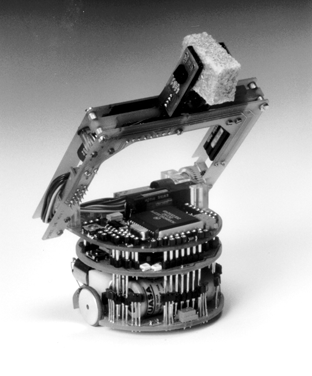
\includegraphics[scale=0.6]{comportamientos/gripperAH.png}
\caption{Robot Khepera con el m\'odulo Gripper}
\label{fig:khepera}
\end{center}
\end{figure}
La base tiene una fuente de luz asociada y el objetivo del
robot es llevar peque\~nos objetos a un lugar de dep\'osito. Se utiliza \emph{aprendizaje por refuerzo} para
asociar las velocidades angulares a los diferentes tama\~nos de las "basuras". Para obtener el comportamiento
deseado se hace uso de \emph{algoritmos gen\'eticos} y \emph{redes neuronales}. Una vez obtenido el mismo mediante
simulaci\'on en Webots, se lo prob\'o en el Khepera f\'isico.
Comparando el trabajo de Stefano Nolfi con el nuestro podemos observar que:
\begin{itemize}

\item{Existencia de un dep\'osito:} Ambos tienen un dep\'osito en el cual dejar la basura recogida y una forma
de identificarla: una fuente de luz usada por Nolfi y en nuestro trabajo, al llegar al final de una determinada
l\'inea de la arena.

\item{Autonom\'ia:} Ambos son aut\'onomos en el sentido que no son manejados por un ente externo. En cuanto
a la recarga de la bater\'ia, Nolfi no explicita si es asistida o no; en nuestro caso, el robot se encarga
de ir a la base de recarga una vez detectada la falta de energ\'ia.

\item{M\'etodo de Recolecci\'on:} En el trabajo de Nolfi se utiliza un m\'odulo agregado al Khepera, que simula
un brazo con dos dedos, la recolecci\'on se realiza juntando ambos y la liberaci\'on se realiza separando ambos.
Nuestro trabajo se basa m\'as en la actividad humana que en el comportamiento humano para realizar este comportamiento,
ya que podr\'ia compararse con un recolector de basura que primero guarda lo encontrado usando una pala en su tacho
y luego descarga su tacho en un dep\'osito de mayor tama\~no.

\item{M\'etodo de aprendizaje:} Nuestro trabajo no utiliza alguna forma de aprendizaje por refuerzo o algoritmo
evolutivo. No es el caso de Nolfi, que utiliza ambas t\'ecnicas para evolucionar el comportamiento deseado.

\item{Robot Utilizado:} Como ya se dijo, Nolfi utiliz\'o un Khepera en la simulaci\'on. En nuestro trabajo
utilizamos un E-puck para la simulaci\'on, una versi\'on nueva del Khepera, pero sin el m\'odulo Gripper.
\begin{figure}[htp]
\begin{center}
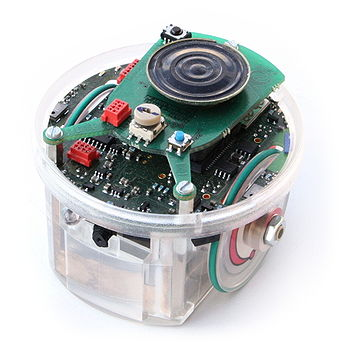
\includegraphics[scale=0.6]{comportamientos/e-puck.png}
\caption{Robot E-puck}
\label{fig:epuck}
\end{center}
\end{figure}

\end{itemize}

\subsubsection{Arquitectura de control para un Robot Aut\'onomo M\'ovil - Neves And Oliveira \cite{Neves97acontrol}}
Neves y Oliveira describen en su trabajo una arquitectura de control basada en comportamientos para un
robot m\'ovil en un ambiente din\'amico, utilizando muchos aspectos de la arquitectura \emph{Subsumption} propuesta
por \emph{Brooks} y que fue usada por nosotros al realizar \'este trabajo explicada en \ref{arq_prop}.
La arquitectura propuesta, o \emph{Control System Arquitecture}, se basa tambi\'en en la teor\'ia de
\emph{The Society of Mind}, escrita por \emph{Minsky}, donde el sistema es visto como una sociedad de agentes,
cada uno con una particular competencia y que colaboran entre ellos para ayudar a la sociedad a alcanzar
su meta.
La arquitectura est\'a compuesta por tres niveles: un nivel reflexivo, uno reactivo, y otro cognitivo, aumentando
la complejidad al igual que el orden en que fueron presentados.
\\
El nivel reflexivo incluye aquellos comportamientos
innatos, es decir, act\'uan directamente como est\'imulo-respuesta. El segundo nivel, el reactivo, est\'a
compuesto por agentes que responden r\'apidamente a los est\'imulos ya que requieren poco nivel de procesamiento.
Finalmente, en el nivel cognitivo, se encuentran los agentes encargados de guiar y administrar los comportamientos
reactivos de forma tal que el robot muestre un comportamiento orientado.
\\
Aunque la arquitectura explicada es similar a la utilizada en nuestro trabajo, \'esta organizaci\'on de los
comportamientos en capas no la utilizamos, aunque podemos divisar que algunos de los comportamientos que propusimos
corresponden a la primera capa de reflexi\'on, como por ejemplo el evitamiento de
obst\'aculos; otros podr\'ian incluirse en la segunda capa de comportamientos reactivos, como lo es deambular y
finalmente en la \'ultima capa estar\'ia el reconocimiento de objectos debido a su gran demanda de procesamiento.

\subsubsection{Path Planning usando Algoritmos Gen\'eticos - Salvatore Candido \cite{salvatore}}
En este paper se describe la utilizaci\'on de algor\'itmos gen\'eticos para resolver el problema de Path Planning.
\'Este problema consiste en armar un plan, una secuencia de acciones de forma tal que a partir de un punto de origen y siguiendo
ese plan, se llegue a un segundo punto, el de destino. Debido a la componente din\'amica de nuestro trabajo, siempre
tratamos de mantener los comportamientos del robot lo m\'as reactivos posibles, por lo que armar un plan no 
ser\'ia el mejor approach para ser utilizado. Por el contrario, el uso de algor\'itmos gen\'eticos puede ser
una herramienta que podr\'ia llegar a ser utilizada en una futura continuaci\'on de nuestro trabajo y que no
utilizamos por el tiempo que estimamos que nos hubiese demandado.

\subsubsection{Navegaci\'on predictiva de un robot aut\'onomo - Foka And Trahanias \cite{Foka02predictiveautonomous}}
La navegaci\'on predictiva nace como una posible soluci\'on al problema de un robot navegando en un ambiente
con muchas personas y obst\'aculos, tal como lo es el ambiente en el cual navegar\'a el robot resultante
de nuestro trabajo.
\\
La forma en que es implementada por los autores es mediante un \emph{POMDP}, es decir, 
un proceso de decisi\'on de markov parcialmente observable. Cabe destacar estas dos \'ultimas palabras, ya
que indican la naturaleza del ambiente: hay incertidumbre o falta de informaci\'on acerca de ciertas variables
del entorno. En este caso, se utiliza el \emph{POMDP} para manejar tanto la navegaci\'on del robot como el
evitamiento de obst\'aculos, un punto en que se diferencia de lo propuesto por nosotros, que es tratar el
\emph{wandering} de forma separada del m\'odulo de evitamiento de obst\'aculos. \'Esto, en parte, se debi\'o
a la arquitectura utilizada y que desde ese punto de vista, ambos comportamientos son muy lejanos.

\subsubsection{Algoritmo de navegaci\'on y evitamiento de obst\'aculos en un entorno desconocido - Clark Et. al \cite{clark}}
En este paper se presentan dos algoritmos complementarios para la navegaci\'on en ese tipo de entornos.
\\
El primero consiste en la navegaci\'on y un mapeo del entorno que garantiza una cobertura completa de una arena
cuyas ubicaciones de la paredes no se conocen \emph{a priori}. Consiste b\'asicamente en un seguimiento de las
paredes complementado por una variaci\'on de \emph{flood filling} para asesgurarse la cobertura completa de la
arena. El algoritmo completo se puede apreciar en la figura \ref{fig:clark}
\begin{figure}[htp]
\begin{center}
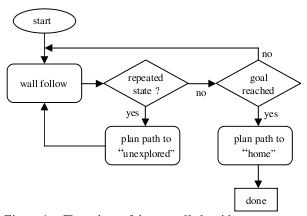
\includegraphics[scale=0.8]{comportamientos/clarkDiagram.png}
\caption{Algoritmo completo}
\label{fig:clark}
\end{center}
\end{figure}
\\
Un aut\'omata con aprendizaje estoc\'astico es el algoritmo que complementa al primero, y su objetivo es
el evitamiento de obst\'aculos. Para \'esto, se utiliza un mecanismo de recompensa/castigo de forma tal
que se adapten las probabilidades de las acciones a tomar. 
\\
En relaci\'on con nuestro trabajo, hay ciertas similitudes y diferencias, enumeradas a continuaci\'on:
\begin{itemize}
\item{}Ambos presentan un mecanismo de "seguimiento de", en nuestro caso lo hacemos con l\'ineas y basuras, en
el paper se utiliza con paredes. Sin embargo, se utilizan para objetivos diferentes. Nosotros lo usamos para
dirigirnos a la base ya que tratamos de mantener el conociemiento que el robot tiene sobre el mundo lo m\'as
acotado posible, o, en el caso de las basuras, para recolectarlas. En el paper se utiliza el mecanismo de seguir
las l\'ineas para obtener un modelo del mundo, algo que puede llegar a servir mucho en ambientes no tan din\'amicos
como el nuestro, raz\'on por la cual no elegimos implementarlo.
\item{}Tambi\'en se coincide en la existencia de un m\'etodo para evitar obst\'aculos. En el paper se implementa como
un aut\'omata que va aprendiendo seg\'un los premios o castigos que recibe; en nuestro caso, el comportamiento es puramente
reactivo y reacciona en base a los valores de los sensores de distancia, pero no tiene memoria.
\end{itemize}

\newpage
\subsection{Arquitectura propuesta}
\label{arq_prop}
Una arquitectura basada en comportamientos define la forma en que los mismos son especificados, desde
su granularidad ( que tan complejo o simple es un comportamiento ), la base para su especificaci\'on,
el tipo de respuesta y la forma en que se coordinan.
\\
La arquitectura que elegimos para desarrollar nuestro trabajo es \emph{Subsumption}, desarrollada por
Rodney Brooks a mediados de 1980. \'Esta arquitectura est\'a basada en comportamientos puramente reactivos,
rompiendo as\'i con el esquema que estaba de moda en la \'epoca de \emph{sensar-planear-actuar}. Algunos
de los principios propuestos que fueron tenidos en cuenta durante el desarrollo de nuestro trabajo son:
\begin{itemize}
\item{}Un comportamiento complejo no es necesariamente el producto de un complejo sistema de control
\item{}El mundo es el mejor modelo del mismo
\item{}La simplicidad es una virtud
\item{}Los sistemas deben ser construidos incrementalmente
\end{itemize}
Cada comportamiento es un par est\'imulo-respuesta. Tal como se observa en la Figura \ref{fig:behaviour},
cada est\'imulo o respuesta puede ser inhibido o suprimida por otros comportamientos activos.
Adem\'as, cada comportamiento recibe una se\~nal de reset, que vuelve al comportamiento que
recibi\'o esta se\~nal a su estado original.
\begin{figure}[htp]
\begin{center}
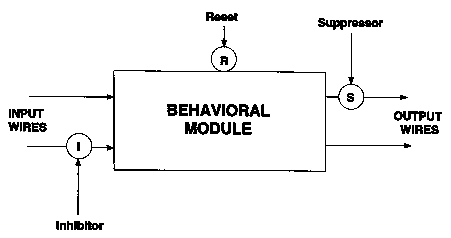
\includegraphics[scale=0.85]{comportamientos/behaviour.png}
\caption{Esquema de comportamiento}
\label{fig:behaviour}
\end{center}
\end{figure}
El nombre \emph{Subsumption} proviene de la forma en que los comportamientos son coordinados entre s\'i. Hay
una jerarqu\'ia donde los comportamientos de la arquitectura tienen mayor o menor prioridad seg\'un su posici\'on.
Los comportamientos de los menores niveles no tienen conocimiento de los comportamientos de las capas de mayor
nivel. Gracias a esto, se puede plantear un dise\~no incremental, brindando flexibilidad, adaptaci\'on y paralelismo
al desarrollo e implementaci\'on de los comportamientos.
\\
La idea a seguir es que el mundo sea el principal medio de comunicaci\'on entre los comportamientos, dado que la respuesta
de un comportamiento ante est\'imulo resulta en un cambio en el mundo y, por lo tanto, en la relaci\'on del robot con el mismo,
ya que el robot en su pr\'oximo paso sensar\'a otro estado del mundo.
\\
El procedimiento b\'asico para dise\~nar y desarrollar comportamientos para robots con esta arquitectura es sencillo:
\begin{enumerate}
\item Especificar cualitativamente la forma en que el mundo responde al mundo, es decir, el comportamiento que realizar\'a.
\item Descomponer la especificaci\'on como un conjunto de acciones disjuntas.
\item Determinar la granularidad del comportamiento, analizando en que nivel de la jerarqu\'ia existente se encontrar\'a y 
cu\'antas acciones disjuntas es necesario llevar a cabo para el cumplimiento de la tarea.
\end{enumerate}

Un ejemplo de \'esta arquitectura se puede observar en \ref{fig:subsumptionExample}. En la misma hay 4 comportamientos:
Homing, Pickup, Avoiding y Wandering. Las l\'ineas que entran a cada comportamiento son los est\'imulos ante los cuales
se activan y las salidas de los mismos son las se\~nales de respuesta correspondientes. La se\~nal de respuesta de la arquitectura
es la l\'inea que sale por la derecha de la caja (Arquitectura) que contiene la relaci\'on entre los comportamientos.
Puede verse como Homing inhibe la salida de Pickup ya que su salida entra al supresor (denotado con un c\'irculo con una S dentro)
de la salida de Pickup y por lo tanto, las salidas de los dem\'as comportamientos, ya que su prioridad es mayor al resto. En el
caso que no est\'en presentes los est\'imulos de Homing, Pickup y Avoiding, no hay inhibici\'on en la salida de Wandering, y por lo
tanto se lleva a cabo el comportamiento de Wandering.
\begin{figure}[htp]
\begin{center}
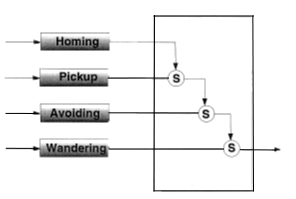
\includegraphics[scale=1.0]{comportamientos/subsumptionExample.png}
\caption{Un ejemplo de Subsumption}
\label{fig:subsumptionExample}
\end{center}
\end{figure}


\newpage

\subsection{Comportamientos e implementaciones}
\label{comportamientos}

Una vez que decidimos utilizar la arquitectura explicada en la secci\'on
\ref{arq_prop} para nuestro proyecto, tuvimos que analizar:
\begin{itemize}
\item{}Forma de implementaci\'on de la arquitectura en c\'odigo
\item{}Comportamientos a realizar
\item{}Ordenes de inhibici\'on y supresi\'on entre los mismos
\item{}Forma de implementaci\'on de los mismos
\item{}Orden de implementaci\'on
\end{itemize}

%Detallar que se hizo con cada item
Para implementar la arquitectura decidimos asignarle un $ID$ num\'erico
diferente a cada comportamiento. Tambi\'en tomamos la decisi\'on de elegir como
comportamiento activo en el instante $t$, aquel comportamiento que est\'e
activo en ese instante y tenga mayor $ID$, suprimiendo as\'i el resto de los
comportamientos (con un $ID$ menor) que podr\'ian estar activos.

%Explicar como se relaciona el requerimiento (robot recolector de basura
%autonomo) con los comportamientos que pusimos
El requerimiento de este proyecto es la realizaci\'on de un robot aut\'onomo
que recolecte basura de su entorno din\'amico pero estructuralmente fijo.
De aqu\'i se infieren algunos de los comportamientos que debe tener el robot:
\begin{itemize}
	\item{\emph{Recolectar basura} (\ref{collect_garbage})}
	\item{\emph{Recargar bater\'ia} (\ref{recharge_battery}):} Por ser
		aut\'onomo, debe poder ser capaz de recargarse s\'olo para poder continuar
		con su actividad.
	\item{\emph{Wandering} (\ref{wandering}):} El robot no es controlado por
		control, ya que	es aut\'onomo, por lo que debe poder recorrer el entorno
		por s\'i mismo.
	\item{\emph{Evitamiento de obst\'aculos} (\ref{avoid_obstacles}):} Debido a
		la naturaleza del entorno, el robot debe ser capaz de navegar sin chocarse
		contra los l\'imites del entorno ni con las personas que circulan por el
		mismo.
\end{itemize}

El comportamiento de recolectar basura y el requerimiento de la autonom\'ia
llevan a su vez a la aparici\'on de m\'as comportamientos: \emph{Descargar
basura} (\ref{unload_garbage}) e \emph{Ir hacia basura} (\ref{go_to_garbage}).
\\
La figura \ref{fig:architecture} muestra los comportamientos implementados y
su orden de jerarqu\'ia. Se puede ver que hay m\'as comportamientos de los
detallados anteriormente. \'Esto se debi\'o a que la forma en que se
implementamos los comportamientos b\'asicos del robot nos requiri\'o el
desarrollo de comportamientos auxiliares.
\\
\begin{figure}[htp]
\begin{center}
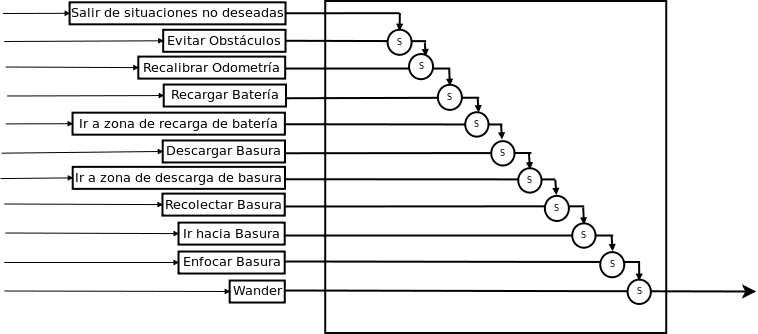
\includegraphics[scale=0.5]{comportamientos/behavioursArchitecture2.png}
\caption{Arquitectura de Comportamientos}
\label{fig:architecture}
\end{center}
\end{figure}
\\
Primero implementamos \emph{Wandering} debido a, en una primera aproximaci\'on,
la sencillez del mismo. Luego implementamos \emph{Evitamiento de obst\'aculos}
para lograr que el robot pueda navegar sin problemas por el arena. Como el
comportamiento de recolectar e ir hacia la basura dependend\'ia del m\'odulo
de reconocimiento de objetos y el mismo estaba siendo desarrollado en paralelo,
se decidi\'o implementar el comportamiento de \emph{Recargar bater\'ia} y
\emph{Descargar basura}. Una vez que tuvimos la primera implementaci\'on
funcional del reconomiento de objetos, procedimos a desarrollar
\emph{Ir hacia basura} y \emph{Recolectar Basura}.
\\
A continuaci\'on detallamos los comportamientos indicados en la figura
\ref{fig:architecture}, as\'i como la implementaci\'on en
\textit{pseudo-codigo} de los mismos y detalles tenidos en cuenta para la
realizaci\'on de los mismos.
%A continuacion vamos a explicar cada comportamiento.....

\subsubsection{Wandering}
\label{wandering}

\paragraph{Detalle del comportamiento} 
Por ser el comportamiento que menor jerarqu\'ia tiene (Ver figura
\ref{fig:architecture}), es el \'unico comportamiento que est\'a activado
ante la ausencia de un est\'imulo, asegurandonos que siempre haya por lo menos
un comportamiento activo.
\\
En una primer aproximaci\'on de \emph{Wandering}, s\'olo nos preocupamos por
ir hacia adelante ya que eventualmente, el robot encuentra un obst\'aculo y
realiza un giro cambiando la direcci\'on del robot.
\\
Los resultados de la simulaci\'on nos indicaron que el robot no recorr\'ia
ciertas zonas o las recorr\'ia despu\'es de un largo tiempo, lo que nos llev\'o
a un segundo approach. El mismo tiene en cuenta el hecho de que el robot posee
una c\'amara y por lo tanto se puede llevar un seguimiento de los lugares que
m\'as recientemente visit\'o o las zonas que hace mucho tiempo no visita.
\\
\'Este approach, en cierta forma, genera un modelo del mundo, un hecho que
conflict\'ua con uno de los principios propuestos a seguir en la secci\'on
\ref{arq_prop}. Para minimizar el conflicto, decidimos mantener al m\'inimo la
informaci\'on almacenada para el funcionamiento del algoritmo, es decir, por
cada zona de arena s\'olo mantenemos el timestamp de la \'ultima vez que el
robot la visit\'o.

\paragraph{Implementaci\'on del comportamiento}

La implementaci\'on del segundo approach, en \emph{pseudo-c\'odigo} es la
siguiente:
\begin{verbatim}
por cada paso
    zona = pedir_zona_vista(camara)
    marcar_zona_como_vista(modelodelmundo,zona)
    ultimazonavisitada = pedir_ultima_zona_visitada(modelodelmundo)
    velocidades = calcular_velocidades_de_ruedas(ultimazonavisitada)
    poner_velocidades_en_ruedas(velocidades)
\end{verbatim}
Para obtener la zona vista por la c\'amara, necesitamos de la altura $C_h$ a la
cual est\'a ubicada la c\'amara en el robot, el campo de visi\'on (de ahora en
adelante \emph{Field of View o FOV}) horizontal $FOV_h$ o vertical $FOV_v$ y
el \'angulo de inclinaci\'on de la c\'amara $ac$. Viendo la figura 
\ref{fig:angleCamera} podemos ver que:

\begin{figure}[htp]
\begin{center}
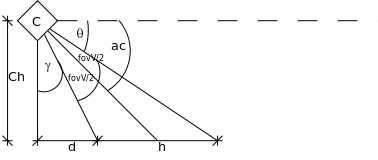
\includegraphics{comportamientos/angleCamera.png}
\caption{Diagrama de posici\'on de la c\'amara}
\label{fig:angleCamera}
\end{center}
\end{figure}

\begin{eqnarray}
ac = \frac{FOV_v}{2} + \theta\\
\gamma + FOV_v + \theta = \frac{\pi}{2}\\
\tan(\gamma) = \frac{d}{C_h}\\
\tan(\gamma+FOV_v) = \frac{d+h}{C_h}
\end{eqnarray}

%En caso de no disponer del $FOV_v$, el mismo se puede obtener de:
%\begin{equation}
%FOV_v = \atan(\frac{ \tan(\frac{FOV_h}{2}) * height}{width} * 2)\\
%\end{equation}
Organizando las ecuaciones, podemos deducir que:

\begin{eqnarray}
\gamma = \frac{\pi}{2} + ac - \frac{FOV_v}{2}\\
\label{eqn:distance_d}
d = \tan(\gamma) * C_h \\
\label{eqn:distance_dh}
d+h = \tan(\gamma+FOV_v) * C_h
\end{eqnarray}

Por lo que obtenemos el \'angulo hasta el inicio de la im\'agen de la c\'amara
$\gamma$ y como consecuencia, la distancia $d$ desde la posici\'on de la
c\'amara hasta el inicio de la im\'agen y $d+h$, la distancia desde la
posici\'on de la c\'amara hasta el final de la im\'agen. Usando \'estos datos,
la posici\'on del robot $P$ y bas\'andonos en la figura \ref{fig:zoneCamera},
podemos obtener los puntos $A$, $B$, $C$ y $D$ del trapezoide que determina la
zona que ve la c\'amara.

\begin{figure}[htp]
\begin{center}
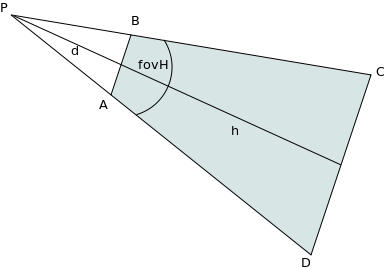
\includegraphics[scale=0.5]{comportamientos/rectangleWander.png}
\caption{Zona vista por la c\'amara}
\label{fig:zoneCamera}
\end{center}
\end{figure}

\subsubsection{Enfocar Basura}
\label{focus_garbage}
Una vez que el m\'odulo de detecci\'on de objetos reconoce algo como basura
(ver secci\'on \ref{algoritmo_vision}), hay que elegir
la forma en que se va a la basura. En la figura \ref{fig:papproachgoto} se
puede ver un primer approach de hacer \'esto. Consiste en primero enfocar la
basura de forma tal que la misma quede en el centro de la imagen de la
c\'amara. De aqu\'i surge el comportamiento \emph{Enfocar Basura}.
\\
Un segundo approach (Figura \ref{fig:sapproachgoto}) no consiste en enfocar la
basura, sino que se idea un arco hacia la misma. \'Esto requiere que se seteen
las velocidades correspondientes a las ruedas de forma tal que la trayectoria
del robot describa dicho arco. Con este segundo approach no existir\'ia el
comportamiento que se est\'a describiendo.
\\
Dado que el primer approach es levemente m\'as simple de implementar, y
teniendo en cuenta el principio enunciado en la secci\'on \ref{arq_prop}
\emph{``La simplicidad es una virtud''}, elegimos implementar el mismo, a
pesar de tener un posible inconveniente, como se puede ver en la figura
\ref{fig:papproachgotoproblem}.
\\
Cuando hay una basura en alguna esquina superior de la imagen de la c\'amara,
y el robot gira sobre s\'i mismo para enfocarla, la basura puede llegar a
perderse por el fondo de la imagen. \'Esto se debe a que la distancia hacia
dichas esquinas es mayor a la distancia hacia el centro del borde superior de
la imagen (Ver figura \ref{fig:zoneCamera}). Decimos que es un ``posible''
problema, ya que una vez que se pierde de vista la basura, el robot no
enfocar\'a m\'as debido a que el est\'imulo desapareci\'o, pero si luego se
dirige hacia adelante (por la activaci\'on de alg\'un otro comportamiento), la
basura volver\'a a aparecer en la imagen, sin desaprovechar la oportunidad de
recogerla.

\begin{figure}[htp]
\begin{center}
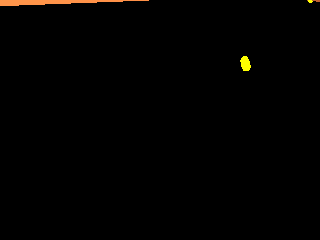
\includegraphics[scale=0.5]{comportamientos/basura.png}
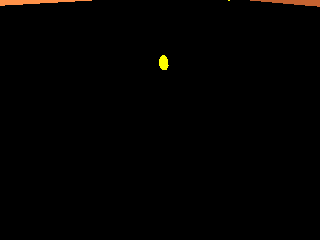
\includegraphics[scale=0.5]{comportamientos/basuraenfocada.png}
\caption{Primer approach de ir a la basura}
\label{fig:papproachgoto}
\end{center}
\end{figure}

\begin{figure}[htp]
\begin{center}
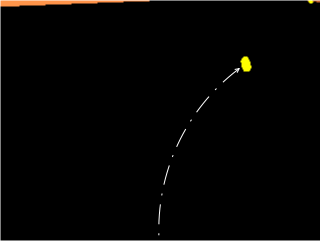
\includegraphics[scale=0.5]{comportamientos/basuraAlt.png}
\caption{Segundo approach de ir a la basura}
\label{fig:sapproachgoto}
\end{center}
\end{figure}

\begin{figure}[htp]
\begin{center}
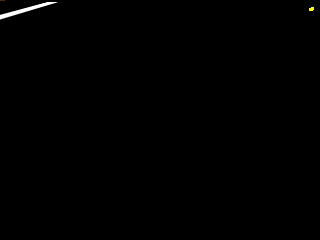
\includegraphics[scale=0.3]{comportamientos/esquina.png}
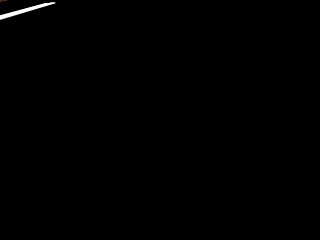
\includegraphics[scale=0.3]{comportamientos/frentemuylejos.png}
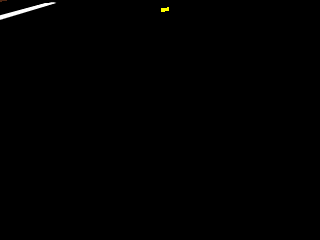
\includegraphics[scale=0.3]{comportamientos/frentelejos.png}
\caption{Posible inconveniente con el primer approach de ir a la basura}
\label{fig:papproachgotoproblem}
\end{center}
\end{figure}

\paragraph{Detalle del comportamiento}
El approach elegido, entonces, se puede describir como:
\begin{itemize}
\item Si la basura est\'a a la izquierda de la im\'agen, se debe girar hacia la
			izquierda
\item Si la basura est\'a a la derecha de la im\'agen, se debe girar hacia la
			derecha
\item Si la basura est\'a en el centro, ya est\'a enfocada
\end{itemize}

%En el caso que haya m\'as de una basura elegimos la m\'as cercana, usando
%c\'alculos detallados a continuaci\'on.
\paragraph{Implementaci\'on del comportamiento}
\label{focus_garbage:impl}
El comportamiento sigue el siguiente \emph{pseudo-codigo}:
\begin{verbatim}
por cada paso
    lista_de_basuras = obtener_lista_de_basuras(modulodereconocimiento)
    basura_mas_cercana = elijo_basura_mas_cercana(lista_de_basuras)
    angulo_a_basura = obtener_angulo(basura_mas_cercana)
    velocidad = VELOCIDAD_BASE * (abs(angulo_a_basura) / (PI/2))
               + VELOCIDAD_BASE_MINIMA

    si angulo_a_basura < 0 entonces
        veloc_izq = -velocidad
        veloc_der = velocidad
    sino
        veloc_izq = velocidad
        veloc_der = -velocidad
    fin_si
    poner_velocidades_en_ruedas(veloc_izq,veloc_der)
\end{verbatim}

Se puede ver que la velocidad de giro del robot es proporcional al m\'odulo del
\'angulo que hay hacia la basura, logrando enfocar m\'as r\'apido cuando el
\'angulo es mayor y tener mayor precisi\'on cuando el \'angulo es m\'as chico,
adem\'as de tener mayor rapidez de enfoque y precisi\'on que si la velocidad de
giro fuera constante.
\\

%%Para obtener el \'angulo y distancia hacia una basura....
%%pasamos de una posicion (x,y) en la imagen a una posicion
%(x,z) en el mundo. teniendo nuestra posicion P, podemos
%calcular la distancia y el angulo
\subsubsection{Ir a Basura}
\label{go_to_garbage}
Luego de la elecci\'on de la forma que se resuelve la situaci\'on de encontrar
una basura (ver \ref{focus_garbage}), el comportamiento de ir a basura es
trivial, ya que la basura, luego de ser enfocada, est\'a delante del robot y lo
\'unico que basta es ir hacia adelante.

\paragraph{Detalle del comportamiento}
El est\'imulo necesario para que este comportamiento est\'e presente est\'a
dado por dos condiciones:
\begin{enumerate}
\item El m\'etodo de reconociemiento de objetos reconoci\'o una basura
\item La basura se encuentra en un entorno del medio horizontal de la imagen de
la c\'amara
\end{enumerate}

\paragraph{Implementaci\'on del comportamiento}
\label{go_to_garbage:impl}
\begin{verbatim}
por cada paso
    distancia = obtener_distancia_a_basura(modulodereconocimiento)
    coeff = (distancia - DIST_MIN)/(DIST_MAX - DIST_MIN)
    veloc_der = VELOCIDAD_MIN*(1 - coeff) + coeff*VELOCIDAD_MAX
    veloc_izq = veloc_der
    poner_velocidades_en_ruedas(veloc_izq,veloc_der)
\end{verbatim}

Al igual que en la implementaci\'on del comportamiento \ref{focus_garbage:impl},
las velocidades que se le otorgan a las ruedas dependen de la distancia
hacia la basura, de forma tal que si una basura est\'a muy lejos, la velocidad
sea mayor y a medida que se va acercando, vaya disminuyendo linealmente.

Dado que la basura se encuentra en un entorno del eje Y en la imagen (Ver figura
\ref{fig:image_coord_conv}b) cometemos un error muy peque\~no al estimar la
distancia a la basura como si estuviera sobre el mismo (asumiendo que la
coordenada X de la basura en la imagen es 0).

Como muestran las figuras \ref{fig:image_coord_conv} y \ref{fig:angleCamera},
el \'angulo vertical hacia el punto m\'as alto de la imagen $(0,C_{rh})$ es 
$\gamma+FOV_v$ y hacia el m\'as bajo, $(0,0)$, el \'angulo es $\gamma$.
De las ecuaciones \eqref{eqn:distance_d} y \eqref{eqn:distance_dh} sabemos
las distancias a los puntos $(0,0)$ (DIST\_MIN) y $(0,C_{rh})$ (DIST\_MAX). 
Entonces, para obtener la distancia $dy$ hacia el punto $(0,y)$ basta con
calcular:
\begin{eqnarray}
y_{angle} = FOV_v * \frac{y}{h} \\
dy = \tan(\gamma + y_{angle}) * C_h \\
\end{eqnarray}

donde $y_{angle}$ es la proporci\'on de $FOV_v$ hacia $y$.
\begin{figure}[htp]
\begin{center}
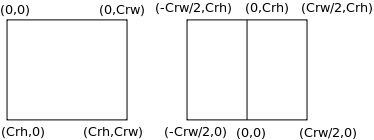
\includegraphics[scale=0.5]{comportamientos/imageCoordsConvertion.png}
\caption{Conversi\'on de coordenadas de imagen de c\'amara}
\label{fig:image_coord_conv}
\end{center}
\end{figure}

\subsubsection{Recolectar Basura}
\label{collect_garbage}
Una vez que el robot llego a estar posicionado para recolectar la basura
deseada, el comportamiento de \emph{recolectar basura} se activa. El mecanismo
para \'esto fue cambiando a lo largo del desarrollo del proyecto.
\\
En un principio pensamos en usar una rampa interna dentro del robot, de forma
tal que la basura suba esa rampa para luego caer en un dep\'osito de basura
interno al robot. Por problemas con la simulaci\'on de este procedimiento, se
busc\'o otro mecanismo.
\\
El mecanismo que elegimos para usar en la simulaci\'on fue el siguiente:
\begin{itemize}
	\item El robot tiene un servo en su parte posterior (debajo de la c\'amara)
	\item Dos paredes delimitan el espacio a lo largo de la direcci\'on que une
			el centro del robot con el servo anteriormente mencionado.
\end{itemize}

\paragraph{Detalle del comportamiento}
La activaci\'on de \emph{recolectar basura} depende de 3 condiciones:
\begin{itemize}
	\item Las dos condiciones impuestas para \emph{ir a basura}
	\item La distancia a la basura elegida para ser recolectada debe ser menor a
			un umbral.
\end{itemize}

Aqu\'i se puede observar que tan importantes son los comportamientos anteriores
para que el robot logre recolectar la basura.
\\
Es importante la elecci\'on del umbral: un valor muy chico puede llevar a que el
comportamiento no se active porque la basura ya no est\'a m\'as en la imagen.
Por otro lado, un valor muy grande causar\'ia que el robot se disponga a
recolectar una basura que est\'a muy lejos y podr\'ia llegar a moverse por
cuestiones propias del ambiente, llevando as\'i a una innecesaria activaci\'on
del comportamiento.

\paragraph{Implementaci\'on del comportamiento}
El \emph{pseudo-codigo} de este comportamiento es el siguiente:

\begin{verbatim}
    distancia = obtener_distancia_a_basura(modulodereconocimiento)
    levantar(servo_delantero)
    recorrerdistancia(distancia)
    cerrar(servo_delantero)
\end{verbatim}

La distancia hacia la basura es obtenida de la misma forma que en la secci\'on
\ref{go_to_garbage:impl}. Levantar y cerrar el servo consiste en setear su
posici\'on en $\frac{\pi}{2}$ y $0$ respectivamente. Para calcular la distancia
recorrida se utiliz\'o la distancia entre la posici\'on del robot en el
instante $t$, $P_r(t)$ y el instante $t+1$, $P_r(t+1)$, ambas dadas por la
odometr\'ia (Ver secci\'on \ref{odometry}). Las diferentes etapas de la
recolecci\'on de una basura se puede ver en la figura \ref{fig:recollection}.

\begin{figure}[htp]
\begin{center}
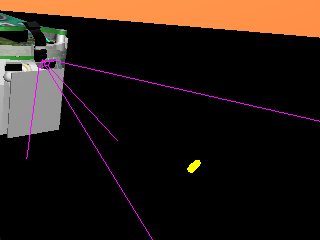
\includegraphics[scale=0.25]{comportamientos/collect1.png}
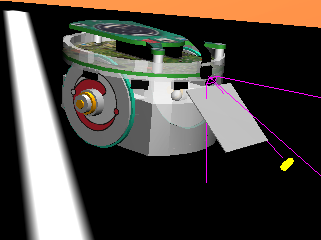
\includegraphics[scale=0.25]{comportamientos/collect2.png}
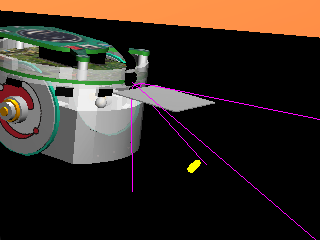
\includegraphics[scale=0.25]{comportamientos/collect3.png}
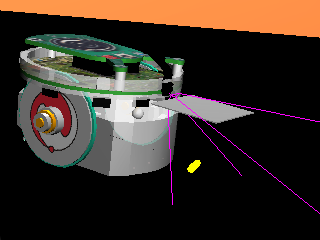
\includegraphics[scale=0.25]{comportamientos/collect4.png}
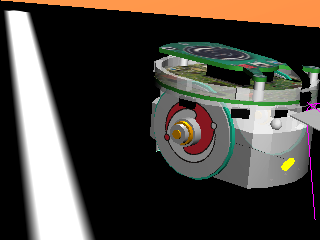
\includegraphics[scale=0.25]{comportamientos/collect5.png}
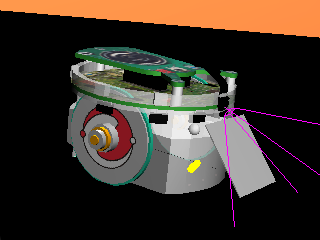
\includegraphics[scale=0.25]{comportamientos/collect6.png}
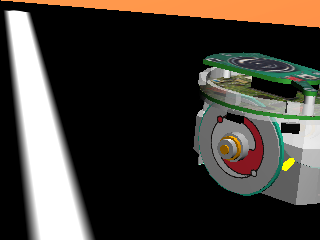
\includegraphics[scale=0.25]{comportamientos/collect7.png}
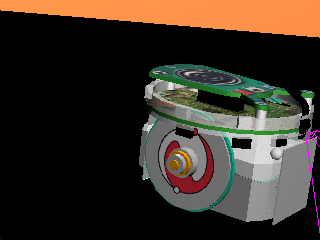
\includegraphics[scale=0.25]{comportamientos/collect8.png}
%
\includegraphics[scale=0.3]{comportamientos/unk.jpg}
\caption{Etapas de recolecci\'on de basura}
\label{fig:recollection}
\end{center}
\end{figure}


\subsubsection{Ir a zona de descarga de basura}
\label{go_to_unload_zone}
Como la capacidad del dep\'osito interno de basura del robot tiene un l\'imite, 
surge como necesidad que el robot sea capaz de ir hacia una zona donde
descargar\'a la basura que contiene, surgiendo as\'i el est\'imulo necesario
para la activaci\'on de este comportamiento.
\\
Para ir hacia dicha zona, decidimos imponerle una condici\'on al
entorno donde el robot actuar\'a. \'Esta condici\'on consiste en poner l\'ineas
de forma tal que si el robot sigue la misma, lo lleve al lugar donde se
encuentra la zona de descarga.
\\
Por lo tanto, para dirigirse a la zona de descarga de basura, es necesario:
\begin{itemize}
	\item Buscar la l\'inea e ir a la misma
	\item Entrar a la l\'inea, de forma tal que el robot y la l\'inea est\'en
				alineados
	\item Seguir la l\'inea
\end{itemize}
Siguiendo con la idea que es mejor descomponer un comportamiento complejo en
otros m\'as simples, decidimos separar el comportamiento de \emph{Ir a zona de
descarga de basura} en 3 comportamientos m\'as simples: \emph{Buscar l\'inea},
\emph{Entrar a la l\'inea} y finalmente \emph{Seguir la l\'inea}.

\paragraph{Buscar l\'inea}
\label{find_line}
Inicialmente, hab\'iamos dispuesto las l\'ineas de forma tal que sigan los
l\'imites de la arena. Entonces para buscar la l\'inea tuvimos que calcular
para cada l\'inea cu\'al es la distancia hacia la misma, luego elegir ir a la
que menor distancia hab\'ia. Adem\'as de ser costoso, este approach ten\'ia un
problema: a veces suced\'ia que al ir hacia una l\'inea, la distancia hacia
otra pasaba a ser m\'as corta y \'esta \'ultima pod\'ia estar m\'as lejos de la
zona de recarga que la primera.
\\
Luego repensamos el problema y nos dimos cuenta que el objetivo era llegar a la
zona de descarga, por lo que decidimos dejar s\'olo 2 las l\'ineas que se
encuentran cerca de la misma, como se puede apreciar en la figura
\ref{fig:arenafinal}. La zona de descarga se ubica cerca de donde se encuentra
el cilindro de color verde.
\\
Para distinguir si el robot est\'a en una l\'inea o no, utilizamos sensores de
piso dispuestos como se muestra en la figura \ref{fig:floorSensors}. Los
sensores se encuentran a una distancia $Fsd$ del centro del robot sobre el eje
$Y$ y los de los costados a una distancia $Fss$ del eje $Y$. La distancia del
sensor del medio hacia el centro del robot es $a$, mientras que la distancia
hacia un sensor del costado es $Fsl = \sqrt{Fsd^2 + Fss^2}$.

\begin{figure}[htp]
\begin{center}
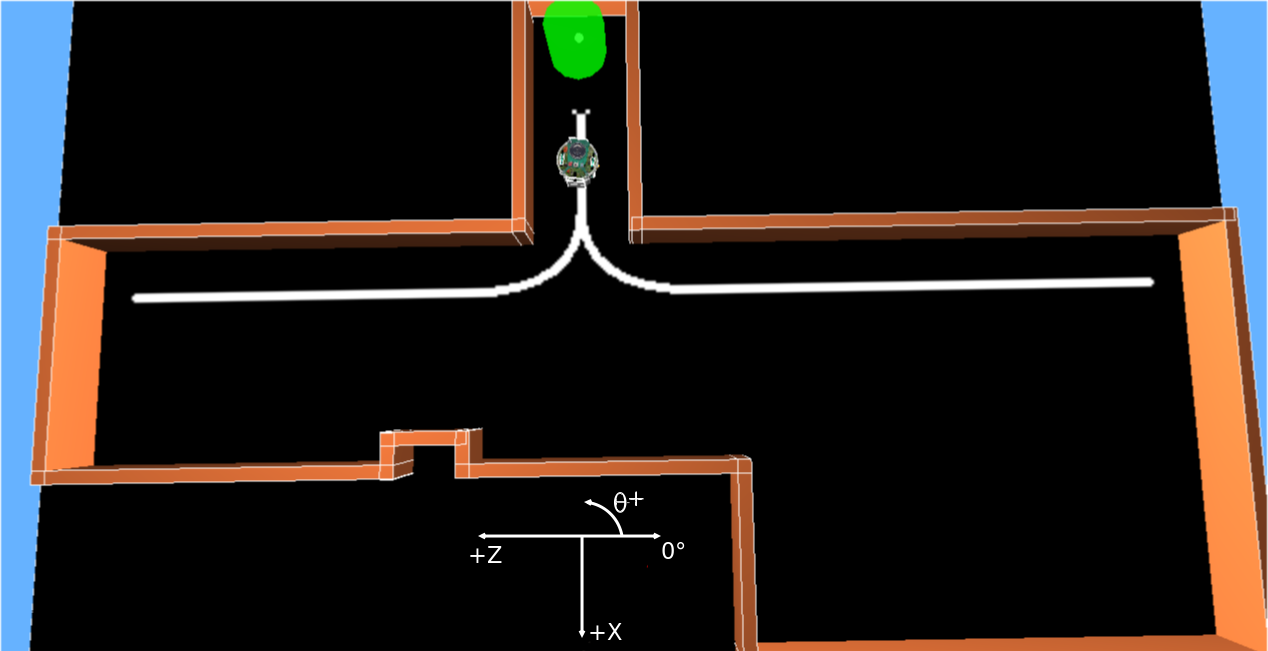
\includegraphics[scale=0.3]{comportamientos/arenafinal.png}
\caption{Arena de simulaci\'on y ejes de coordenadas}
\label{fig:arenafinal}
\end{center}
\end{figure}

\begin{figure}[htp]
\begin{center}
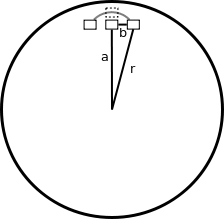
\includegraphics[scale=1.0]{comportamientos/floorSensors.png}
\caption{Disposici\'on de sensores de piso}
\label{fig:floorSensors}
\end{center}
\end{figure}

\subparagraph{Detalle del comportamiento}
La decisi\'on de dejar s\'olo dos l\'ineas, acompa\~nada por la elecci\'on de
la ubicaci\'on de la zona de descarga, nos facilit\'o la composici\'on de
\'este comportamiento.
\\ Como se ve en la figura \ref{fig:arenafinal}, para ir a la l\'inea se debe
girar hasta tener un \'angulo de $\frac{\pi}{2}$ y luego ir hacia adelante.

%Describir la eleccion de las distancias de las lineas hacia las paredes

\subparagraph{Implementaci\'on del comportamiento}
El \emph{pseudo-codigo} de este comportamiento es sencillo, ya que
no requiere c\'alculos extras:

\begin{verbatim}
por cada paso
    angulo_actual = obtener_angulo_actual(odometria)
    si esta_en_un_entorno_de(angulo_actual,PI/2) entonces
        si angulo_actual > PI/2 && angulo_actual < 3PI/2 entonces
            giro_para_la_derecha
        sino
            giro_para_la_izquierda
        fin si
    sino
        voy_hacia_linea
    fin si
\end{verbatim}

Hicimos la verificaci\'on de que el \'angulo est\'e entre $\frac{\pi}{2}$ y
$\frac{3\pi}{2}$ para evitar girar m\'as de $\pi$, girando a la izquierda o a
la derecha dependiendo cual sea el caso. Para ver esto m\'as claramente,
veamos que sucediese si no estuviera:
\begin{verbatim}
    si esta_en_un_entorno_de(angulo_actual,PI/2) entonces
        giro_para_la_izquierda
    sino
\end{verbatim}
En el caso que el angulo actual sea $\pi$, el robot girar\'ia un total de
$\frac{3\pi}{2}$ hasta llegar al \'angulo destino $\frac{\pi}{2}$, cuando en
realidad girando para el sentido contrario s\'olo tendr\'ia que girar
$\frac{\pi}{2}$.
\\
Se puede observar en el c\'odigo usamos datos calculados por la odometr\'ia, en
este caso, la orientaci\'on actual del robot. El lector se podr\'ia preguntar:
``Si la odometr\'ia tiene la posici\'on actual del robot, ?`porqu\'e no se
usaron los datos de la misma para ir hacia la base?''. En principio, esto
requiere que el robot tenga conocimiento acerca de la ubicaci\'on de la base.
Por otro lado, se hubiera tenido que utilizar alg\'un algoritmo de
\emph{Path Planning} para realizar el recorrido, algo que no concuerda con
la arquitectura elegida. Es importante destacar el uso de datos calculados por
la odometr\'ia porque si la misma llega a tener un error grande, puede llevar a
una activaci\'on err\'onea de comportamientos. En la secci\'on
\ref{odometry:problems} se puede ver la incidencia de un error grande de la
odometr\'ia en el comportamiento emergente del robot.

\paragraph{Entrar a l\'inea}
\label{enter_line}
\subparagraph{Detalle del comportamiento}

Para seguir la l\'inea, es necesario que primero el robot est\'e posicionado
sobre ella y alineado con la misma. Tambi\'en se necesita que la direcci\'on
del robot sea la que lo lleve hacia la zona de descarga, por lo que una vez en
la l\'inea, el robot deber\'a girar dependiendo de que lado se encuentre la
misma (Ver figura \ref{fig:arenafinal}).

\subparagraph{Implementaci\'on del comportamiento}
\begin{verbatim}
    angulo_final = obtener_angulo_final(obtener_linea(odometria))
    tita = atan(dist_sens_piso_X,dist_sens_piso_Y)
    si (esta_en_la_linea(sensor_piso(DERECHA))) entonces
        tita = -tita
    fin si
    si (esta_en_la_linea(sensor_piso(MEDIO))) entonces
        tita = 0
    fin si

    si (tita != 0) entonces
        girar(tita)
    fin si

    distancia_a_recorrer = dist_sens_piso_Y;
    si (tita != 0) entonces
        distancia_a_recorrer = sqrt(dist_sens_piso_X^2 + dist_sens_piso_Y^2)
    fin si

    recorrer(distancia_a_recorrer)

    angulo_actual = obtener_angulo(odometria)

    girar(normalizar(angulo_actual - angulo_final))
\end{verbatim}

% Explicar el porque del primer giro
% Relacionarlo con la figura fig:floorSensors
El primer giro del robot es para lograr que el robot quede con el sensor de
piso del medio sobre la l\'inea. Como mostramos en la figura
\ref{fig:floorSensorsStates}, en el caso (a) y (b) el robot girar\'a de forma
tal que llegue un caso parecido al (c) ya posiblemente el sensor del medio no
estar\'a en la l\'inea. Notar que si el sensor del medio est\'a en la l\'inea,
entonces el robot no gira, cualquiera sea el estado de los sensores de los
costados. El \'angulo que debe girar est\'a dado por $\theta = \arctan
(\frac{Fss}{Fsd})$ (Ver figura \ref{fig:floorSensors}) o $-\theta$ seg\'un
cual sea el sensor que est\'e sobre la l\'inea.

\begin{figure}[htp]
\begin{center}
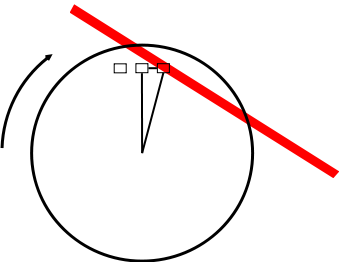
\includegraphics[scale=0.4]{comportamientos/floorSensorsLine.png}
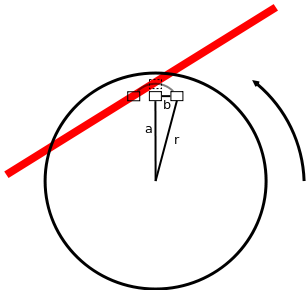
\includegraphics[scale=0.4]{comportamientos/floorSensorsLine1.png}
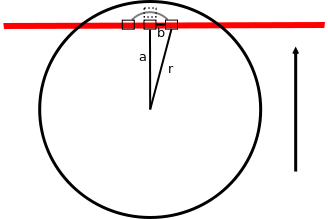
\includegraphics[scale=0.4]{comportamientos/floorSensorsLine2.png}
\caption{Posibles estados iniciales de entrar a la l\'inea}
\label{fig:floorSensorsStates}
\end{center}
\end{figure}


% Explicar el porque del recorrido de la distancia 
% Relacionarlo con la figura fig:floorSensors
Luego del posible giro para lograr que el sensor de piso del medio quede sobre
la l\'inea, se recorre una distancia de $Fsd$, en el caso que el robot no haya
girado anteriormente, o $Fsl$ en el caso que s\'i lo haya hecho. El motivo de
este trayecto es que el centro del robot quede sobre la l\'inea, como muestra
la figura \ref{fig:positioned}. De \'esta forma, s\'olo queda girar nuevamente
hacia el \'angulo que se quiera. Si la l\'inea es la izquierda, entonces el
robot deber\'a girar hasta que su orientaci\'on sea $0$, o $\pi$ en el caso
que la l\'inea sea la derecha.

\begin{figure}[htp]
\begin{center}
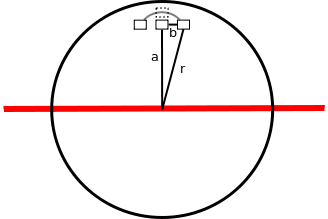
\includegraphics[scale=0.4]{comportamientos/floorSensorsLine3.png}
\caption{Centro del robot sobre la l\'inea y posibles giros}
\label{fig:positioned}
\end{center}
\end{figure}

\paragraph{Seguir l\'inea}
\label{follow_line}
Una vez que el robot est\'a posicionado y con el sensor del medio sobre la
l\'inea, s\'olo basta con seguirla para llegar hacia la zona deseada. \'Este
comportamiento es sencillo de desarrollar.

\subparagraph{Detalle del comportamiento}
Para lograr que el robot siga la l\'inea el objetivo es tratar de mantener
s\'olo el sensor del medio sobre la l\'nea. Entonces, basta con analizar que se
debe hacer en los siguientes casos:
\begin{enumerate}
	\item El sensor de la derecha est\'a sobre la l\'inea
	\item El sensor de la izquierda est\'a sobre la l\'inea
\end{enumerate}
En el primer caso, se debe lograr sacar el sensor de la derecha de la l\'inea,
describiendo un peque\~no arco hacia ese lado. El segundo caso es an\'alogo:
para sacar el sensor de la izquierda de la l\'inea se debe seguir una
trayectoria con un peque\~no \'angulo hacia la izquierda. 

\subparagraph{Implementaci\'on del comportamiento}
El \emph{pseudo-c\'odigo} es simple:
\begin{verbatim}
por cada paso
    veloc_izq = veloc_der = VELOC_SEGUIR_LINEA
    si (esta_en_la_linea(sensor_piso(IZQUIERDA))) entonces
        veloc_izq *= (1 - FACTOR_DE_GIRO)
        veloc_der *= (1 + FACTOR_DE_GIRO)
    fin si
    si (esta_en_la_linea(sensor_piso(DERECHA))) entonces
        veloc_izq *= (1 + FACTOR_DE_GIRO)
        veloc_der *= (1 - FACTOR_DE_GIRO)
    fin si
    poner_velocidades_en_ruedas(veloc_izq,veloc_der)
\end{verbatim}

\subsubsection{Descargar Basura}
\label{unload_garbage}
Una vez que el robot logr\'o llegar a la zona de descarga de basura, debe
descargarla. Para \'esto decidimos ubicar un servo en la parte trasera del
robot, con la misma idea del servo en la parte posterior utilizado para
recolectar.

\paragraph{Detalle del comportamiento}
Para descargar la basura el robot debe posicionarse de forma tal que la
compuerta de descarga quede adyacente a la zona. Dado que para llegar a la
misma el robot sigui\'o la l\'inea, al finalizar va a estar orientado con un
\'angulo en un entorno de $\frac{\pi}{2}$, mirando la zona de descarga. Como el
servo de descarga se encuentra en la parte trasera, deber\'a realizar un giro
para luego poder descargar la basura.
\paragraph{Implementaci\'on del comportamiento}
\begin{verbatim}
    posicionarse()
    levantar(servo_trasero)
    recorrerdistancia(ANCHO_ROBOT)
    cerrar(servo_trasero)
\end{verbatim}

\subsubsection{Ir a base de recarga de bater\'ia}
\label{go_to_recharge}
Ayudados por la elecci\'on que tomamos de poner la zona de descarga de basura
muy cercana a la zona donde se recarga la bater\'ia, decidimos utilizar la
misma estrategia de seguir la l\'inea para llegar hacia la misma.
\\
La diferencia
entre ambos casos es el est\'imulo ante el cual se activan. En el caso de
ir a la zona de descarga, el est\'imulo proviene del sensor del dep\'osito
interno de basura que indica que el mismo est\'a lleno. En el caso de ir
a la base de recarga de bater\'ia, el est\'imulo para la activaci\'on depende
de los valores de dos sensores de bater\'ia que indican bater\'ia baja:
\begin{itemize}
	\item El sensor de la bater\'ia del robot, de donde se alimentan los sensores,
			actuadores y motores.
	\item El sensor de la computadora que corre el controlador.
\end{itemize}

\subsubsection{Cargar Bater\'ia}
\label{recharge_battery}
\paragraph{Detalle del comportamiento}
\paragraph{Implementaci\'on del comportamiento}
\begin{verbatim}
    posicionarse()
    mientras(bateria_no_llena(BATERIA_ROBOT)
            o bateria_no_llena(BATERIA_PC)) hacer

        esperar()
    fin mientras
\end{verbatim}

\begin{comment}

\subsubsection{Recalibrarse}
\label{recalibrate}
\paragraph{Detalle del comportamiento}
\paragraph{Implementaci\'on del comportamiento}

\end{comment}

\subsubsection{Evitar Obst\'aculos}
\label{avoid_obstacles}
\emph{Evitar obst\'aculos} es uno de los comportamientos con mayor jerarqu\'ia
en la arquitectura que elegimos. Su nivel se debe a la importancia que tiene
en un ambiente estructurado pero din\'amico como es el elegido. El objetivo
del robot es facilitar una tarea, sin entorpecer el tr\'ansito de personas.
\\
\paragraph{Detalle del comportamiento}
Para lograr tener conocimiento sobre la proximidad de un obst\'aculo, utilizamos
sensores de proximidad explicados en \ref{sensores de proximidad}.
Dependiendo de la proximidad sensada por un sensor, el robot deber\'a alejarse
de ese lado para evitar un posible choque. La activaci\'on del comportamiento
depender\'a entonces de un valor menor del sensor que haga que la distancia
hacia un obst\'aculo lleve al robot a quedarse estancado o le imposibilite
moverse.
\paragraph{Implementaci\'on del comportamiento}
La implementaci\'on de \'este comportamiento la hicimos utilizando una
red neuronal sin capas ocultas (ver figura \ref{fig:redN}) usando los sensores
de distancia como entradas y las 2 neuronas de salida indicando los valores a
ser seteados a los motores de las ruedas.
\\
Notar que hay conexiones tanto inhibitorias como excitatorias. Como es de
esperarse, ambos sensores traseros (4 y 5) exitan a ambos motores. Distinto es
el caso de los sensores del lado izquierdo (5, 6 y 7) que exitan el motor
ubicado de su lado e inhiben el motor del lado opuesto, de forma tal que el
robot gire para el lado opuesto de la ubicaci\'on de los sensores. La misma
idea se sigue con los sensores (0, 1 y 2) ubicados en el costado derecho del
robot.
\\
Luego de entrenar la red, obtuvimos los siguientes valores para los pesos de la
misma:

\begin{table}[ht]
	\begin{center}
		\begin{tabular}{ | c | c | c | c | c | c | c | c | c | }
			\hline 
			Rueda & $W_0$ & $W_1$ & $W_2$ & $W_3$ &  $W_4$ & $W_5$ & $W_6$ & $W_7$ \\
			\hline\hline
			Izquierda & -0.9 & -0.85 & -0.2 & 0.6 & 0.5 & 0.35 & 0.8 & 0.6 \\
			\hline
			Derecha & 0.9 & 0.85 & 0.2 & 0.6 & 0.5 & -0.35 & -0.8 & -0.6 \\
			\hline
		\end{tabular}
	\end{center}
	\label{pesos_obstaculo} 
	\caption{Asignaci\'on de pesos para evitar obst\'aculos}
\end{table}
Se puede ver que los pesos que influyen en el motor de una rueda influyen
con igual fuerza pero distinto signo en el motor de la rueda contraria.
\\
Este comportamiento, en \emph{pseudo-codigo} puede verse como:
\begin{verbatim}
por cada paso
    veloc_izq = suma(coeficiente(RUEDA_IZQ)(SENSOR_I) * VALOR(SENSOR_I))
    veloc_izq *= FACTOR_DE INCIDENCIA
    veloc_der = suma(coeficiente(RUEDA_DER)(SENSOR_I) * VALOR(SENSOR_I))
    veloc_der *= FACTOR_DE INCIDENCIA
    poner_velocidades_en_ruedas(veloc_izq,veloc_der)
\end{verbatim}

\begin{figure}[htp]
\begin{center}
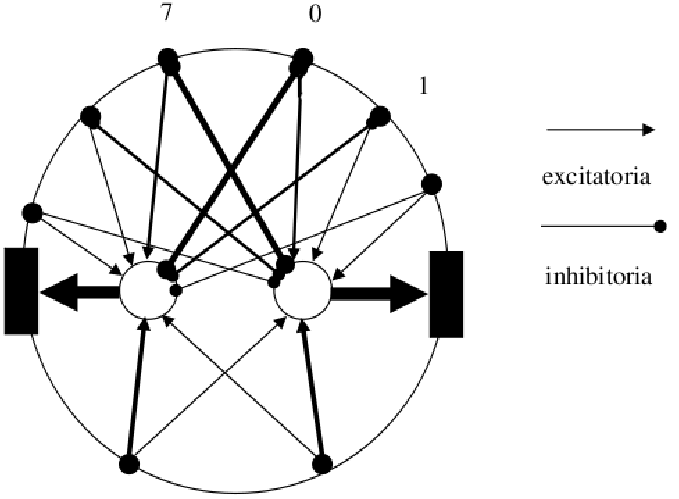
\includegraphics[scale=0.4]{comportamientos/red.png}
\caption{Red neuronal entre los sensores de distancia y los motores}
\label{fig:redN}
\end{center}
\end{figure}

\subsubsection{Salir de situaciones no deseadas}
\label{out_of_unwanted_situations}
\emph{Salir de situaciones no deseadas} surgi\'o como un comportamiento
para ayudar al objetivo de la autonom\'ia del robot. A medida que fuimos
corriendo las simulaciones, observamos que hab\'ia situaciones donde corr\'ia
peligro la autonom\'ia del robot. Un ejemplo de estas situaciones es el caso
donde se ``activan mutuamente'' entre dos comportamientos.
\\
Para ver esto m\'as claramente, supongamos dos comportamientos $A$ y $B$ con
nivel en la jerarqu\'ia $N(A)$ y $N(B)$, siendo $N(A) > N(B)$. Si la respuesta
a un est\'imulo de $A$ lleva a la activaci\'on de $B$ y a la desactivaci\'on de
$A$ y luego la respuesta de $B$ lleva a la activaci\'on de $A$, podr\'ia llegar
a entrarse en un ciclo si es que esta situaci\'on se da por un tiempo
prolongado. El mayor peligro para la autonom\'ia se corre cuando $A$ es el
comportamiento de \emph{evitar obst\'aculos} y $B$ es el comportamiento de
\emph{ir a zona de recarga de bater\'ia} ya que el robot podr\'ia terminar
qued\'andose sin bater\'ia en ese ciclo.
\paragraph{Detalle del comportamiento}
Las situaciones no deseadas se dan la mayor\'ia de los casos cuando un
comportamiento hace girar al robot hacia un lado y el otro comportamiento hacia
el lado contrario, aproximadamente en la misma magnitud. \'Esto quiere decir
que la posici\'on del robot se mantiene alrededor de un punto por un per\'iodo
prolongado de tiempo, por lo que decidimos tomar este hecho como est\'imulo
para la activaci\'on de este comportamiento.
\\
La respuesta del comportamiento es, entonces, girar un \'angulo que cambie la
direcci\'on del robot y adem\'as, que la suma de esa magnitud no sea
peri\'odica.
\'Esta \'ultima condici\'on se pide por el siguiente escenario:
\begin{itemize}
	\item Los comportamientos $A$ y $B$ se ``activan mutuamente'' cuando la
		orientaci\'on del robot es $0$.
	\item Los comportamientos $C$ y $D$ se ``activan mutuamente'' cuando la
		orientaci\'on del robot es $\pi$.
	\item La respuesta de \emph{salir de situaciones no deseadas} es girar un
		\'angulo $\pi$.
\end{itemize}

\paragraph{Implementaci\'on del comportamiento}
\begin{verbatim}
    angulo_actual = obtener_angulo_actual(odometria)
    nuevo_angulo = angulo_actual + ANGULO_A_SUMAR
    girar(nuevo_angulo)
\end{verbatim}



\newpage
\subsection{Odometr\'ia}
\label{odometry}
Para saber donde se encuentra el robot en cierto momento, se utiliza odometr\'ia.
\\
\'Esta se basa en la medici\'on de las cuentas dadas por un motor para obtener el desplazamiento realizado 
por la rueda asociada al mismo. Dado que el motor que usamos fue un motor diferencial para cada rueda,
\'esto es posible de realizar.
\\
A diferencia de los m\'etodos de posicionamiento absoluto, la odometr\'ia
da una estimaci\'on del desplazamiento \emph{local} a la ubicaci\'on anterior del robot, por lo cual \emph{un error}
en una estimaci\'on \emph{se propaga} hacia las siguientes estimaciones. 
\\
Para calcular la posici\'on en el instante n $P_n$ y la orientaci\'on $O_n$ en base a la posici\'on en el 
instante (n-1) $P_{n-1}$ y la correspondiente orientaci\'on $O_{n-1}$, usamos las siguientes f\'ormulas:
\begin{eqnarray}
d_l = \frac{(e_l(n) - e_l(n-1)) * R_l}{EncRes} \\
d_r = \frac{(e_r(n) - e_r(n-1)) * R_r}{EncRes} \\
lc = \frac{d_r + d_l}{2} \\
P_n = P_{n-1} + (lc * \cos{O_{n-1}},lc * \sin{O_{n-1}}) \\
O_n = O_{n-1} + \frac{d_r - d_l}{dbw}
\end{eqnarray}
donde $d_l$ y $d_r$ son las distancias recorridas por las ruedas izquierda y derecha respectivamente. Ambas
son calculadas teniendo en cuenta los valores anteriores y actuales de los encoders $e_i(n)$, el radio de la rueda $R_i$ y
la resoluci\'on del encoder $EncRes$. $dbw$ es la distancia entre ruedas.
\\
Los errores que influyen en el c\'alculo de la odometr\'ia pueden ser de dos tipos:

\begin{itemize}

\item{Sistem\'aticos:} Son aquellos que pueden ser corregidos o tenidos en cuenta para disminuir el error.

\item{No sistem\'aticos:} Son aquellos que pueden intentarse corregir pero \emph{no} eliminar.

\end{itemize}

Decidimos tener en cuenta dos errores sistem\'aticos para disminuir el error en la odometr\'ia :
\begin{itemize}
\item{Incerteza sobre la distancia entre las ruedas ($dbw$)}
\item{Ruedas con radios diferentes ($R_l$ y $R_r$)}
\end{itemize}
Tuvimos en cuenta estos errores dado que son los que m\'as contribuyen al error acumulado a lo
largo del trayecto del robot.
Para corregir \'estas fuentes de error, utilizamos el \emph{test del camino
bidireccional describiendo un cuadrado} (UMBmark)\footnote{http://www-personal.umich.edu/~johannb/Papers/umbmark.pdf}.
Dado que en el momento de realizar el test no hab\'ia un robot f\'isico, decidimos realizar el test sobre
un e-puck simulado en Webots.
As\'i fuimos obteniendo los valores de correcci\'on para los di\'ametros de las ruedas $c_i$ y la correci\'on
sobre la distancia entre las ruedas $c_{dbw}$ hasta que el error sistem\'atico m\'aximo dejara de disminuir. En la
figura \ref{fig:errsist} se puede ver c\'omo disminuye el error a lo largo de las iteraciones.

\begin{figure}[htp]
\begin{center}
%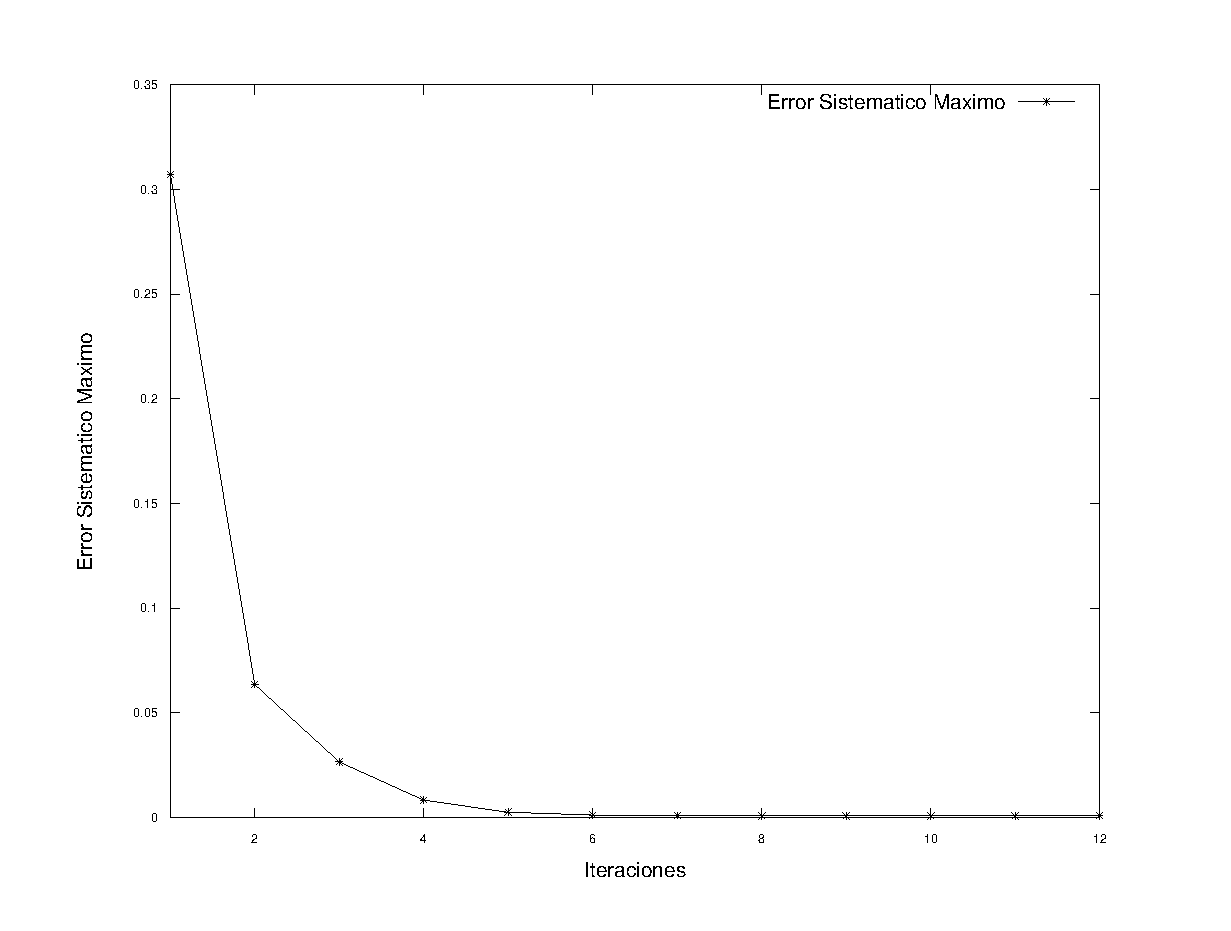
\includegraphics[scale=0.6]{comportamientos/errsist.eps}
\caption{Error Sistem\'atico M\'aximo a lo largo de las iteraciones}
\label{fig:errsist}
\end{center}
\end{figure}

En la \'ultima iteraci\'on obtuvimos los coeficientes de correcci\'on $c_l = 0.99998703$, $c_r = 1.00001297$
y $c_{dbw} = 1.092171094$ para ruedas con radio $R_l = R_r = 0.205$, una distancia entre ruedas de $0.052$ y
una resoluci\'on de encoder $EncRes = 159.23$.

\newpage
\subsection{Interfaces con hardware y m\'odulo de reconocimiento de objetos}
\label{interfaces}
Decidimos hacer que el controlador encargado de realizar los comportamientos sea independiente
de la forma con la que se implemente el hardware y la forma con que se implemente el reconocimiento
de los objetos. Para \'esto definimos interfaces, de forma tal que el controlador las mismas
y tanto el hardware como el m\'odulo de reconocimiento de objetos puedan cambiar su implementaci\'on
pero brindando siempre la informaci\'on que necesita el controlador para poder realizar
los comportamientos. \'Esta decisi\'on nos posibilit\'o realizar un controlador que sea capaz de ser
ejecutado tanto en Webots, donde se hizo el desarroll\'o, como en la base real del robot. Cabe aclarar
que el traspaso de la simulaci\'on a la realidad no es instant\'anea, ya que hay que calibrar los dispositivos,
realizar nuevamente la odometr\'ia, entre otras cosas, pero el trabajo demandado es mucho menor ya
que una correcci\'on en la l\'ogica de los comportamientos se puede observar tanto en un simulador como
en la realidad.

\subsubsection{Interfaz con hardware}
La interfaz con el hardware se basa en tener clases encargadas de obtener los valores de los sensores
o del accionar de los actuadores.
\\En la implementaci\'on de la interfaz que corrimos en Webots, hic\'imos
llamadas al controlador del simulador, que utiliza sensores y actuadores simulados.
\\En la implementaci\'on que se comunica con el robot f\'isico,
las llamadas las hicimos a un servidor encargado de enviar y recibir paquetes del protocolo descripto
en la secci\'on \ref{protocolo} a trav\'es del puerto serial.
\\De est\'a forma es cuesti\'on de decidir que implementaci\'on se usa en base a si se quiere
correr en un simulador como Webots, o en el robot f\'isico. Si se quisiese usar otro simulador
u otro tipo de hardware, s\'olo hace falta implementar la interfaz que cumpla con lo establecido e
indicarle a la capa de comportamientos que la utilice para realizar su ejecuci\'on.

\subsubsection{Interfaz con m\'odulo de reconocimiento de objetos usando Visi\'on}
Dado que el desarrollo de los comportamientos lo hicimos separado del desarrollo del
m\'odulo que reconoce objetos utilizando una c\'amara, decidimos hacer una interfaz de
forma tal que se puedan desarrollar de forma paralela.
Como el controlador de comportamientos es \textbf{usuario} del m\'odulo de reconocimiento,
necesita saber en un instante de tiempo $t$, que objetos est\'an siendo reconocidos. Para \'esto
el m\'odulo debe tener una fuente de informaci\'on, en este caso, una c\'amara dado que se usa
Visi\'on.
\\
Desde el punto de vista de la anatom\'ia, \'esto se puede ver como los ojos (c\'amara), la parte del cerebro
encargada de analizar el est\'imulo recibido por los mismos (m\'odulo de reconocimiento) y la parte del cerebro
encargada de analizar los est\'imulos y realizar las acciones (controlador de comportamientos). Si se hubiese
usado alg\'un tipo de conjunto de sensores t\'actiles para reconocer objetos (mano), en vez de visi\'on, 
el m\'odulo de reconocimiento de objetos bien podr\'ia analizar la informaci\'on que ellos proveen e
informar al controlador sobre su an\'alisis.
\\
\'Esta analog\'ia puede llevar a pensar que los sensores de distancia u otros dispositivos que usamos
en este desarrollo bien podr\'ian formar parte de otro m\'odulo, y no se estar\'ia equivocado. La raz\'on
por la cual el m\'odulo de visi\'on est\'a separado y el resto de los sensores no, es que el procesamiento
de una secuencia de im\'agenes es muy complejo y pesado, como se muestra en la secci\'on \ref{vision}.

\newpage
\subsection{Resultados obtenidos}
\label{results}

\subsubsection{Tiempo promedio en recolectar basura}
%Calcular t min, con un escenario donde las basuras las pongo apenas sale de la base
%Calcular t max, con un escenario donde las basuras estan lo m\'as lejos de la base posible

\subsubsection{Tiempo promedio de wandering}
%(Tiempo en que est\'a activo el wandering)/(Tiempo total de simulaci\'on)

\subsubsection{Distribuci\'on de tiempos entre los diferentes comportamientos}
%(tiempo de comportamiento i)/(Tiempo total de simulaci\'on)

\subsubsection{Relaci\'on (t\_cargando + t\_ir a base) / tiempo total}
%T busqueda basura/ ( t a base + tiempo carga bateria + t salir base )

\subsubsection{Porcentaje de espacio cubierto}
%esp_cub / (esp_cub + esp_nocub)

\subsubsection{Tiempo cubrir toda la arena}

\newpage
\subsection{Conclusi\'on}
\label{comp_conclusion}
Conclusi\'on de comportamientos

